\section{Our Approach}

\subsection{Core Pig Latin Features}
\begin{frame}{Core Pig Features}
\begin{itemize}
	\item \textbf{Programs specify queries over relations:} Designed to
	concisely facilitate common data transformation tasks.
	\item \textbf{Programs manipulate aggregate non-atomic types:} e.g. bags
	and tuples.
	\item \textbf{Programs use UDFs from environment.}
	\item \textbf{Programs specify data flow via statements:} A sequence of
	statements define dependencies between queries via var assignments and uses.
	\item \textbf{Programs are parallelizable/distributable:} Part of a long
	history in data flow and query-oriented programming.
\end{itemize}
\end{frame}

\subsection{Formalism}
\begin{frame}{Conventions}
\centering
	\begin{flushleft}
		T \quad : a type\newline
		S \quad : a type that satisfies schema type\newline
		c \quad : an integer to denote column offset\newline
		x, y : identifiers\newline
		\textGamma \quad : Context\newline
 		s \quad : a statement\newline
 		q \quad : a term of query form\newline
 		$\vdash$ S c T : column c in Schema S has type T\newline
 		+++ : Schema Concatenation\newline
 		*** : Schema constructed from a pair of types\newline
 		::= : Assignment of statement to ID \newline
 		;; : Sequence of Statements
	\end{flushleft}
\end{frame}

\begin{frame}{Grammar: Terms For Logical Plan}
\centering
%	\begin{flushleft}
%	$ \texttt{tm} := \qquad\qquad\qquad\qquad\qquad\:\: \texttt{Terms}\hfill$\\
%	$ \quad \mid \texttt{t\_filter}\hfill \texttt{Query Filter}\hfill$\\
%   	$ \quad \mid \texttt{t\_foreach} \hfill \texttt{Query ForEach}\hfill$\\
%    $ \quad \mid \texttt{t\_group} \hfill \texttt{Query Group}\hfill$\\
%    $ \quad \mid \texttt{t\_join} \hfill \texttt{Query Join}\hfill$\\
%    $ \quad \mid \texttt{t\_load} \hfill \quad\quad\:\: \texttt{Load Statement}\hfill$\\
%   	$ \quad \mid \texttt{t\_assign} \hfill \qquad\qquad\quad \texttt{Assignment Statement}\hfill$\\
%    $ \quad \mid \texttt{t\_seq} \hfill \qquad\qquad\qquad\quad\quad \texttt{Sequence of Statements}\hfill$\\
%    $ \quad \mid \texttt{t\_store} \hfill \quad\quad\:\: \texttt{Store Statement}\hfill$\\
%	\end{flushleft}
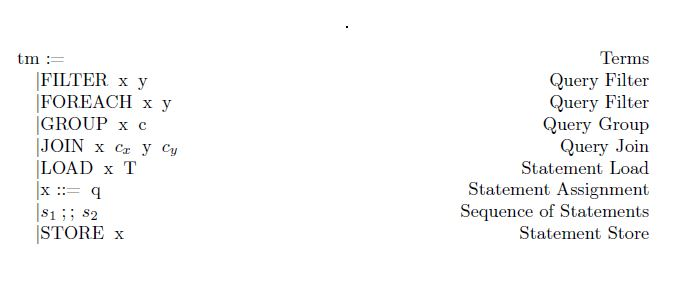
\includegraphics[scale=0.6]{Images/Grammar/Terms.JPG}
\end{frame}


\begin{frame}{Grammar: Terms For Physical Plan}
\centering
%	\begin{flushleft}
%	$ \texttt{tm} := \qquad\qquad\qquad\qquad\qquad\:\: \texttt{Terms}\hfill$\\
%	$ \quad \mid \texttt{t\_filter}\hfill \texttt{Query Filter}\hfill$\\
%   	$ \quad \mid \texttt{t\_foreach} \hfill \texttt{Query ForEach}\hfill$\\
%    $ \quad \mid \texttt{t\_lrearrange} \hfill \texttt{Query Local ReArrange}\hfill$\\
%    $ \quad \mid \texttt{t\_grearrange} \hfill \texttt{Query Global ReArrange}\hfill$\\
%    $ \quad \mid \texttt{t\_package} \hfill \texttt{Query Package}\hfill$\\
%    $ \quad \mid \texttt{t\_load} \hfill \quad\quad\:\: \texttt{Load Statement}\hfill$\\
%   	$ \quad \mid \texttt{t\_assign} \hfill \qquad\qquad\quad \texttt{Assignment Statement}\hfill$\\
%    $ \quad \mid \texttt{t\_seq} \hfill \qquad\qquad\qquad\quad\quad \texttt{Sequence of Statements}\hfill$\\
%    $ \quad \mid \texttt{t\_store} \hfill \quad\quad\:\: \texttt{Store Statement}\hfill$\\
%	\end{flushleft}
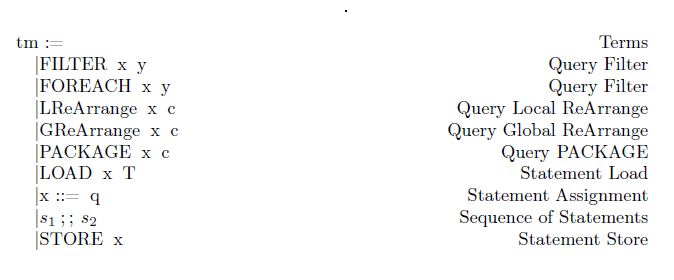
\includegraphics[scale=0.6]{Images/Grammar/Terms_Physical.JPG}
\end{frame}

\begin{frame}{Grammar: Schema Types}
\centering
%	\begin{flushleft}
%	$ schema := \hfill \quad Schema \:Types\hfill$\\
%	$ \quad \mid \texttt{STNil}\hfill \texttt{{Unit Type}}\hfill$\\
%   	$ \quad \mid \texttt{STyPair} \hfill \texttt{Tuple of Column and Schema}\hfill$\\
%
%	$ \texttt{schema} := \hfill \quad\texttt{Schema Types}\hfill$\\
%	$ \quad \mid \texttt{STNil}\hfill \texttt{{Unit Type}}\hfill$\\
%   	$ \quad \mid \texttt{STyPair} \hfill \texttt{Tuple of Column and Schema}\hfill$\\
%
%	\end{flushleft}
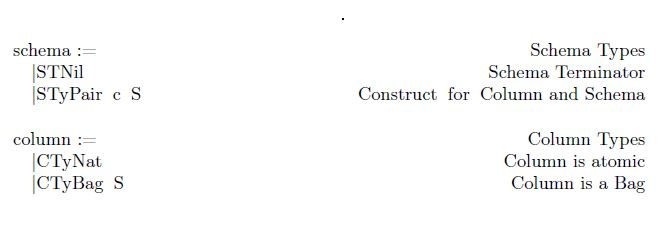
\includegraphics[scale=0.6]{Images/Grammar/Schema.JPG}
\end{frame}


\begin{frame}{Grammar: Relations}
\centering
%	\begin{mathpar}
%		\inferrule* [Right=\texttt{T\_Package}]
%          		{\Gamma \vdash \texttt{x = S} \\ \texttt{schema \:S} \\\\
%          		schema\_column\_has\_type \:S \:c \\\\
%				S' = TInt ::: (TBag S) \\ \texttt{schema \:S'}}
%          		{\Gamma \vdash \texttt{Package \:x c} \in \texttt{S'} }
%	\end{mathpar}
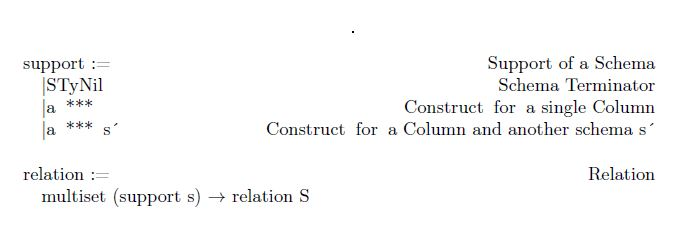
\includegraphics[scale=0.6]{Images/Grammar/Relation.JPG}
\end{frame}

\begin{frame}{Grammar: Types}
\centering
%	\begin{flushleft}
%	$ \texttt{ty} := \qquad\qquad\qquad\qquad\quad\quad\:\: \texttt{Types}\hfill$\\
%	$ \:\:\: \mid \texttt{TUnit}\hfill \texttt{Unit Type}\hfill$\\
%   	$ \:\:\: \mid \texttt{TFn} \hfill\qquad\quad\:\: \texttt{Function Type}\hfill$\\
%    $ \:\:\: \mid \texttt{TPred} \hfill\qquad\quad \texttt{Predicate Type}\hfill$\\
%    $ \:\:\: \mid \texttt{TNil} \hfill \qquad\qquad\qquad\qquad\:\:\: \texttt{Schema Tuple Terminator}\hfill$\\
%    $ \:\:\: \mid \texttt{TCons} \hfill \qquad\qquad\qquad\quad\:\: \texttt{Schema Tuple Extension}\hfill$\\
%   	$ \:\:\: \mid \texttt{TInt} \hfill \qquad\qquad\qquad\qquad\quad \texttt{Atomic Schema Attribute}\hfill$\\
%    $ \:\:\: \mid \texttt{TBag} \hfill \quad\qquad\qquad\qquad\qquad\: \texttt{Compound Schema Attribute}\hfill$\\
%	\end{flushleft}
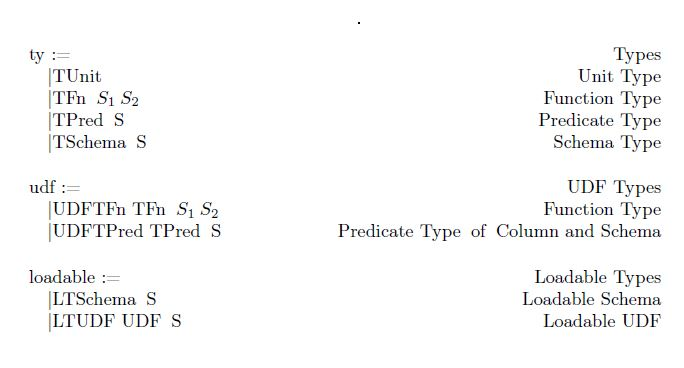
\includegraphics[scale=0.6]{Images/Grammar/Types.JPG}
\end{frame}

\subsection{Typing Rules for Logical Plan}
\begin{frame}{Typing Rules: Queries}
\centering
%	\begin{mathpar}
%		\inferrule* [Right=\texttt{T\_Filter}]
%          		{\Gamma \vdash \texttt{x = S} \\ \texttt{schema \:S} \\
%          		\Gamma \vdash \texttt{y = Pred \:S}}
%          		{\Gamma \vdash \texttt{FILTER \:x, y} \in \texttt{S} }
%		\hva \and
%		\inferrule* [Right={\textbf{T\_ForEach}}]
%          		{schema \:S_1 \\ schema \:S_2 \\\\
%				\Gamma \vdash x = S_1 \\ \Gamma \vdash y = Fn\: S_1\:S_2}
%				{\Gamma \vdash FOREACH \:x\:y \in S }
%	\end{mathpar}
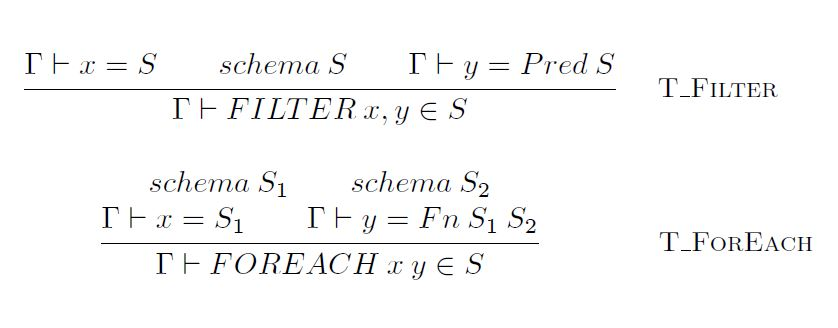
\includegraphics[scale=0.4]{Images/TypingRules/FilterForeach.JPG}
\end{frame}

\begin{frame}{Typing Rules: Queries(continued...)}
\centering
%	\begin{mathpar}
%		\inferrule* [Right=\textbf{T\_Group}]
%          		{\Gamma \vdash x = S \\\\
%          		schema \:S \\ schema \:S' \\\\
%          		schema\_column\_has\_type \:S \:c \\\\
%          		S' = TInt ::: (TBag \:S)}
%          		{\Gamma \vdash GROUP \:x \:c \in S' }
%	\end{mathpar}
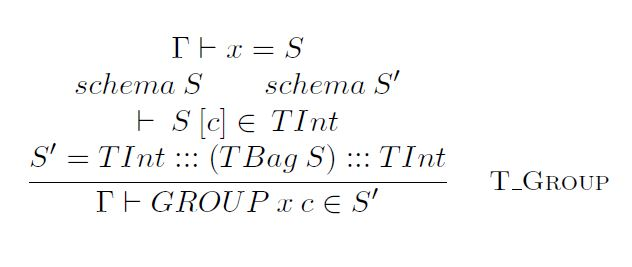
\includegraphics[scale=0.4]{Images/TypingRules/Group.JPG}
\end{frame}

\begin{frame}{Typing Rules: Queries(continued...)}
\centering
%	\begin{mathpar}
%		\inferrule* [Right=\textbf{T\_Join}]
%          		{\Gamma \vdash x = S_1 \\ \Gamma \vdash y =  S_2 \\\\
%          		schema\:S_1 \\ schema \:S_2 \\\\
%		 		schema\_column\_has\_type \:S_1 \:c_x \\\\
%		 		schema\_column\_has\_type \:S_2 \:c_y \\\\
%		 		concatenated\_schema \:S_1\:S_2\:S_3}
%		 		{\Gamma \vdash JOIN \:x \:c_x \:y \:c_y \in S_3 }
%	\end{mathpar}
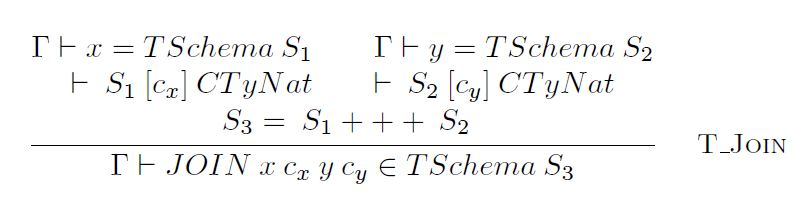
\includegraphics[scale=0.4]{Images/TypingRules/Join.JPG}
\end{frame}

\begin{frame}{Typing Rules: Statements}
\centering
%	\begin{mathpar}
%		\inferrule* [Right=\textbf{T\_Load}]
%          		{\Gamma \vdash x = None \\ loadable\_ty\: T}
%          		{\Gamma \vdash LOAD \:x\:T \in TUnit }
%		\hva \and
%		\inferrule* [Right=\textbf{T\_Assign}]
%          		{\Gamma \vdash x = None \\ \Gamma \vdash q = S \\schema \:S}
%          		{\Gamma \vdash ASSIGN \:x \:q \in TUnit }
%		\hva \and
%		\inferrule* [Right=\textbf{T\_Store}]
%				{\Gamma \vdash x = S \\ schema \:S}
%				{\Gamma \vdash STORE \:x \in TUnit }
%	\end{mathpar}
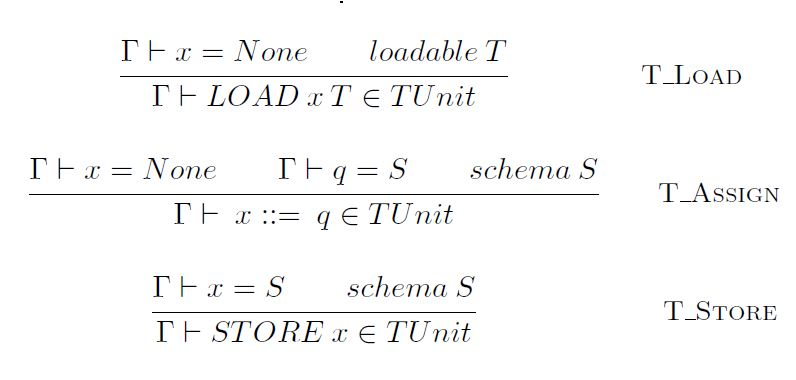
\includegraphics[scale=0.4]{Images/TypingRules/Load_Assign_Store.JPG}
\end{frame}

\begin{frame}{Typing Rules: Statements (continued...)}
\centering
%	\begin{mathpar}
%		\inferrule* [Right=\textbf{T\_SeqLoad}]
%          		{s_1 = LOAD \:x \:T \\ \Gamma \vdash s_1 \in TUnit \\\\
%          		\Gamma, x:T \vdash s_2 \in TUnit }
%          		{\Gamma \vdash SEQ \:s_1 \:s_2 \in TUnit }
%
%		\hva \and
%		\inferrule* [Right=\textbf{T\_SeqAssign}]
%          		{s_1 = ASSIGN \:x \:q \\\\
%          		\Gamma \vdash q = S \\ schema \:S \\\\
%          		\Gamma \vdash s_1 \in TUnit \\ \Gamma, x:S \vdash s_2 \in TUnit}
%          		{\Gamma \vdash SEQ \:s_1 \:s_2 \in TUnit }
%	\end{mathpar}
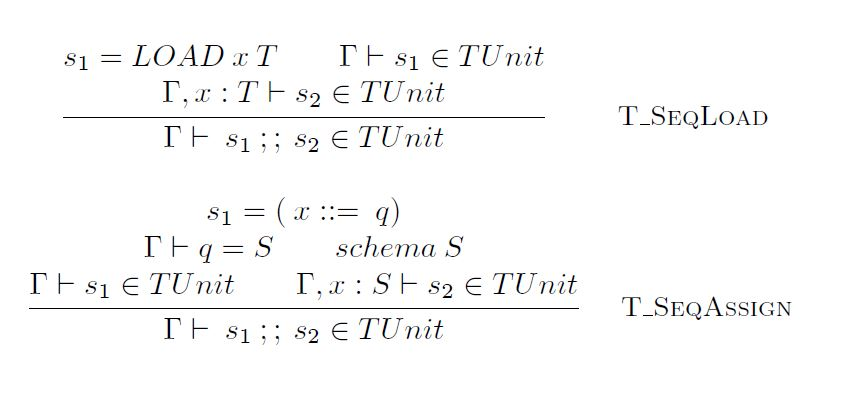
\includegraphics[scale=0.4]{Images/TypingRules/SEQ1.JPG}
\end{frame}

\begin{frame}{Typing Rules: Statements (continued...)}
\centering
%	\begin{mathpar}
%		\inferrule* [Right= \textbf{T\_SeqStore}]
%          	{s_1 = STORE \:x \\\\
%          	\Gamma \vdash x = S \\ schema \:S  \\\\
%			\Gamma \vdash s_1 \in TUnit \\ \Gamma \vdash s_2 \in TUnit }
%			{\Gamma \vdash SEQ \:s_1 \:s_2 \in TUnit }
%	\end{mathpar}
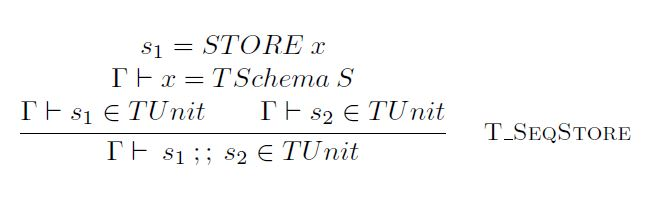
\includegraphics[scale=0.4]{Images/TypingRules/SEQ2.JPG}
\end{frame}

\subsection{Typing Rules for Physical Plan}
\begin{frame}{Typing Rules: Queries}
\centering
%	\begin{mathpar}
%		\inferrule* [Right=\texttt{T\_LReArrange}]
%          		{\Gamma \vdash \texttt{x = S} \\ \texttt{schema \:S} \\\\
%          		schema\_column\_has\_type \:S \:c}
%          		{\Gamma \vdash \texttt{LReArrange \:x c} \in \texttt{S} }\\
%		\inferrule* [Right=\texttt{T\_GReArrange}]
%          		{\Gamma \vdash \texttt{x = S} \\ \texttt{schema \:S} \\\\
%          		schema\_column\_has\_type \:S \:c}
%          		{\Gamma \vdash \texttt{GReArrange \:x c} \in \texttt{S} }
%	\end{mathpar}
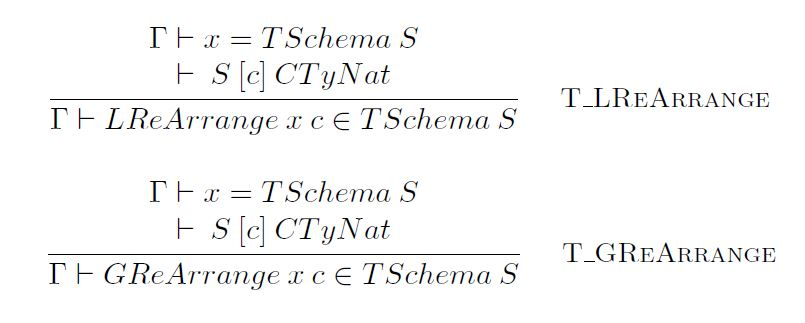
\includegraphics[scale=0.4]{Images/TypingRules/ReArrange.JPG}
\end{frame}

\begin{frame}{Queries(continued...)}
\centering
%	\begin{mathpar}
%		\inferrule* [Right=\texttt{T\_Package}]
%          		{\Gamma \vdash \texttt{x = S} \\ \texttt{schema \:S} \\\\
%          		schema\_column\_has\_type \:S \:c \\\\
%				S' = TInt ::: (TBag S) \\ \texttt{schema \:S'}}
%          		{\Gamma \vdash \texttt{Package \:x c} \in \texttt{S'} }
%	\end{mathpar}
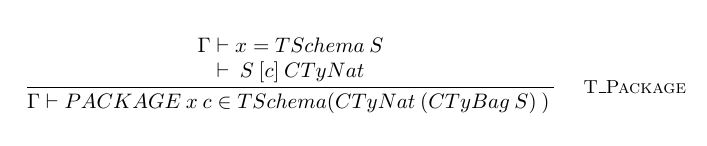
\includegraphics[scale=0.4]{Images/TypingRules/Package.JPG}
\end{frame}

\begin{frame}{Semantics: Representing Relations with multiset}
\centering
  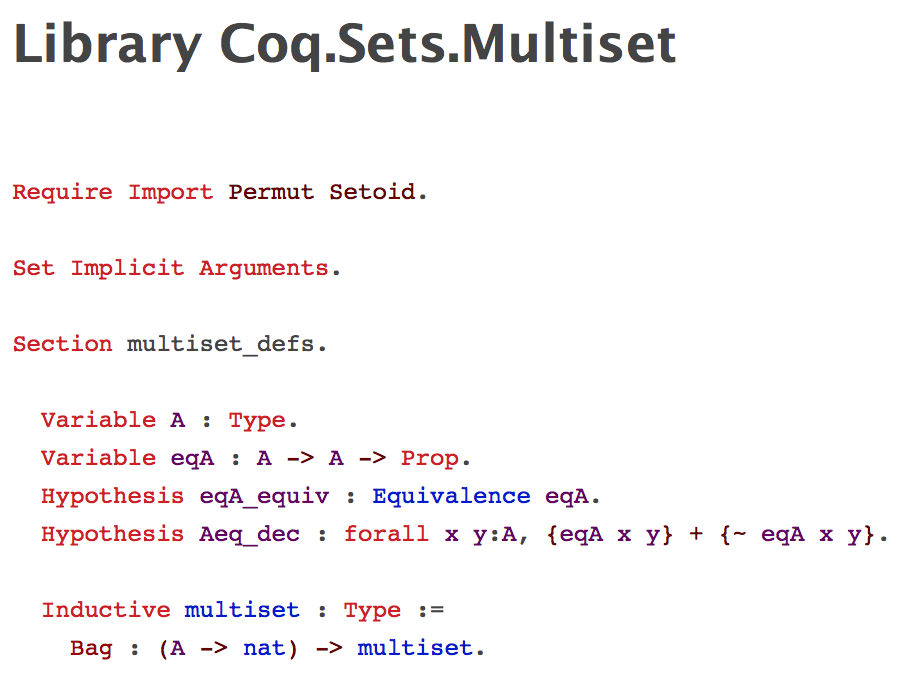
\includegraphics[scale=0.5]{CoqIDE/Semantics/Multisets.png}
\end{frame}

\begin{frame}{Semantics: Four Key Specification Properties}
\centering
  \begin{enumerate}
  \item \texttt{filtered}
	\item \texttt{mapped}
	\item \texttt{grouped}
	\item \texttt{joined}
  \end{enumerate}
\end{frame}

\begin{frame}{Semantics: The \texttt{filtered} Specification}
\centering
  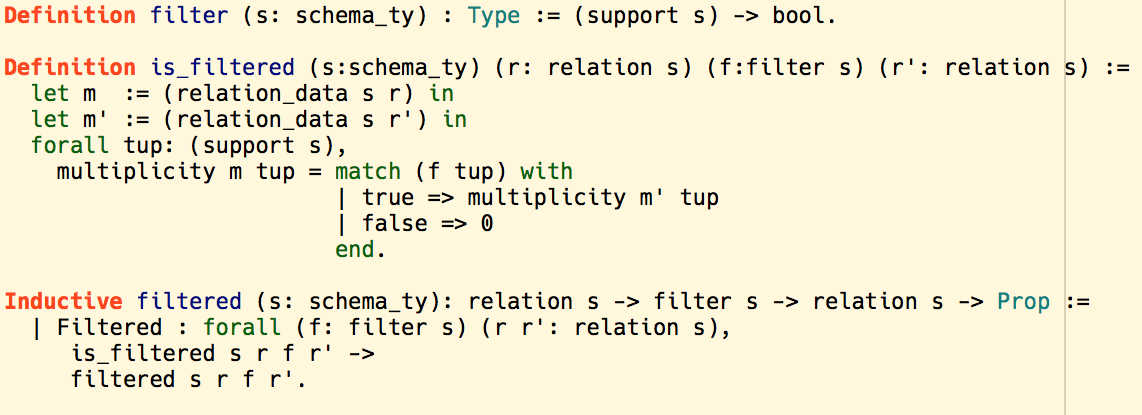
\includegraphics[]{CoqIDE/Semantics/filtered.png}
\end{frame}

\begin{frame}{Semantics: The \texttt{mapped} Specification}
\centering
  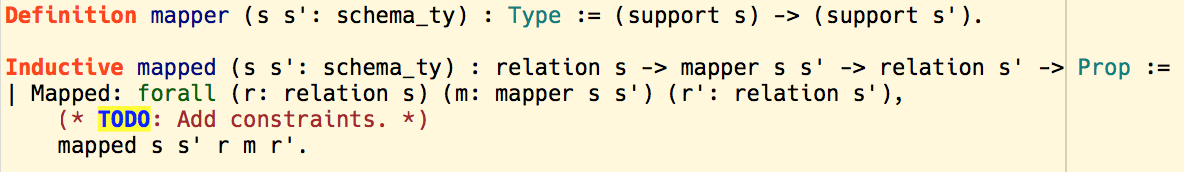
\includegraphics[]{CoqIDE/Semantics/mapped.png}
\end{frame}

\begin{frame}{Semantics: The \texttt{grouped} Specification}
\centering
  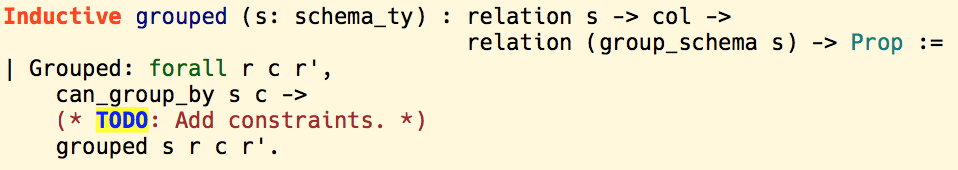
\includegraphics[]{CoqIDE/Semantics/grouped.png}
\end{frame}

\begin{frame}{Semantics: The \texttt{joined} Specification}
\centering
  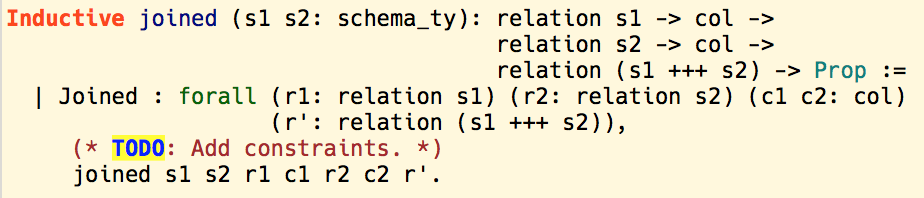
\includegraphics[]{CoqIDE/Semantics/joined.png}
\end{frame}
